\documentclass[11pt]{article}

\usepackage[a4paper,margin=1in]{geometry}
\usepackage{booktabs}
\usepackage{graphicx}
\usepackage{hyperref}
\usepackage{natbib}
\usepackage{siunitx}

\graphicspath{{../outputs/figures/}}

\title{Mitigating Native Class Imbalance in TCGA-UT with Frozen Pathology Features}
\author{}
\date{}

\begin{document}
\maketitle

\begin{abstract}
Class imbalance is a central obstacle in computational pathology because clinically relevant cohorts often follow long-tailed disease distributions. This study evaluates mitigation strategies for native TCGA-UT classification using a shared frozen Virchow2 feature representation. The experiment compares feature-space probes, sampling strategies, loss reweighting, focal losses, hybrid sampling-loss combinations, and set-learning variants under the same train, validation, and test splits. The goal is to identify which methods improve minority-class recognition without obscuring majority-class trade-offs.
\end{abstract}

\section{Introduction}
Computational pathology classifiers are frequently trained on datasets where common tumor types dominate rare entities. Under this regime, aggregate accuracy can hide poor minority-class behavior, and evaluation must emphasize classwise recall, macro-averaged metrics, and calibration-aware views \citep{saini2023tacklingClass,zhang2023deepLong,mosquera2024classImbalance}. TCGA-UT is a useful test bed because it contains many tumor classes and can be studied with frozen pathology foundation-model features.

This paper studies mitigation methods on the native TCGA-UT distribution rather than constructing imbalance artificially. All evaluated methods use the same Virchow2 feature representation \citep{vorontsov2024virchow,zimmermann2024virchow2}, which isolates the effect of the downstream imbalance strategy.

\section{Dataset Exploration}
The analysis starts by building a manifest that maps native TCGA-UT feature files to slide identifiers and cancer types. The manifest is used to quantify class counts, feature coverage, and imbalance ratio before training. Figure~\ref{fig:class-distribution} shows the native class distribution once generated.

\begin{figure}[ht]
  \centering
  \IfFileExists{../outputs/figures/class_distribution.png}{
\includegraphics[width=\linewidth]{class_distribution.png}}{\fbox{\parbox{0.85\linewidth}{Class-distribution figure generated by \texttt{scripts/prep/explore.py}.}}}
  \caption{Native TCGA-UT slide counts by cancer type.}
  \label{fig:class-distribution}
\end{figure}

\begin{figure}[ht]
  \centering
  \IfFileExists{../outputs/figures/long_tail_profile.png}{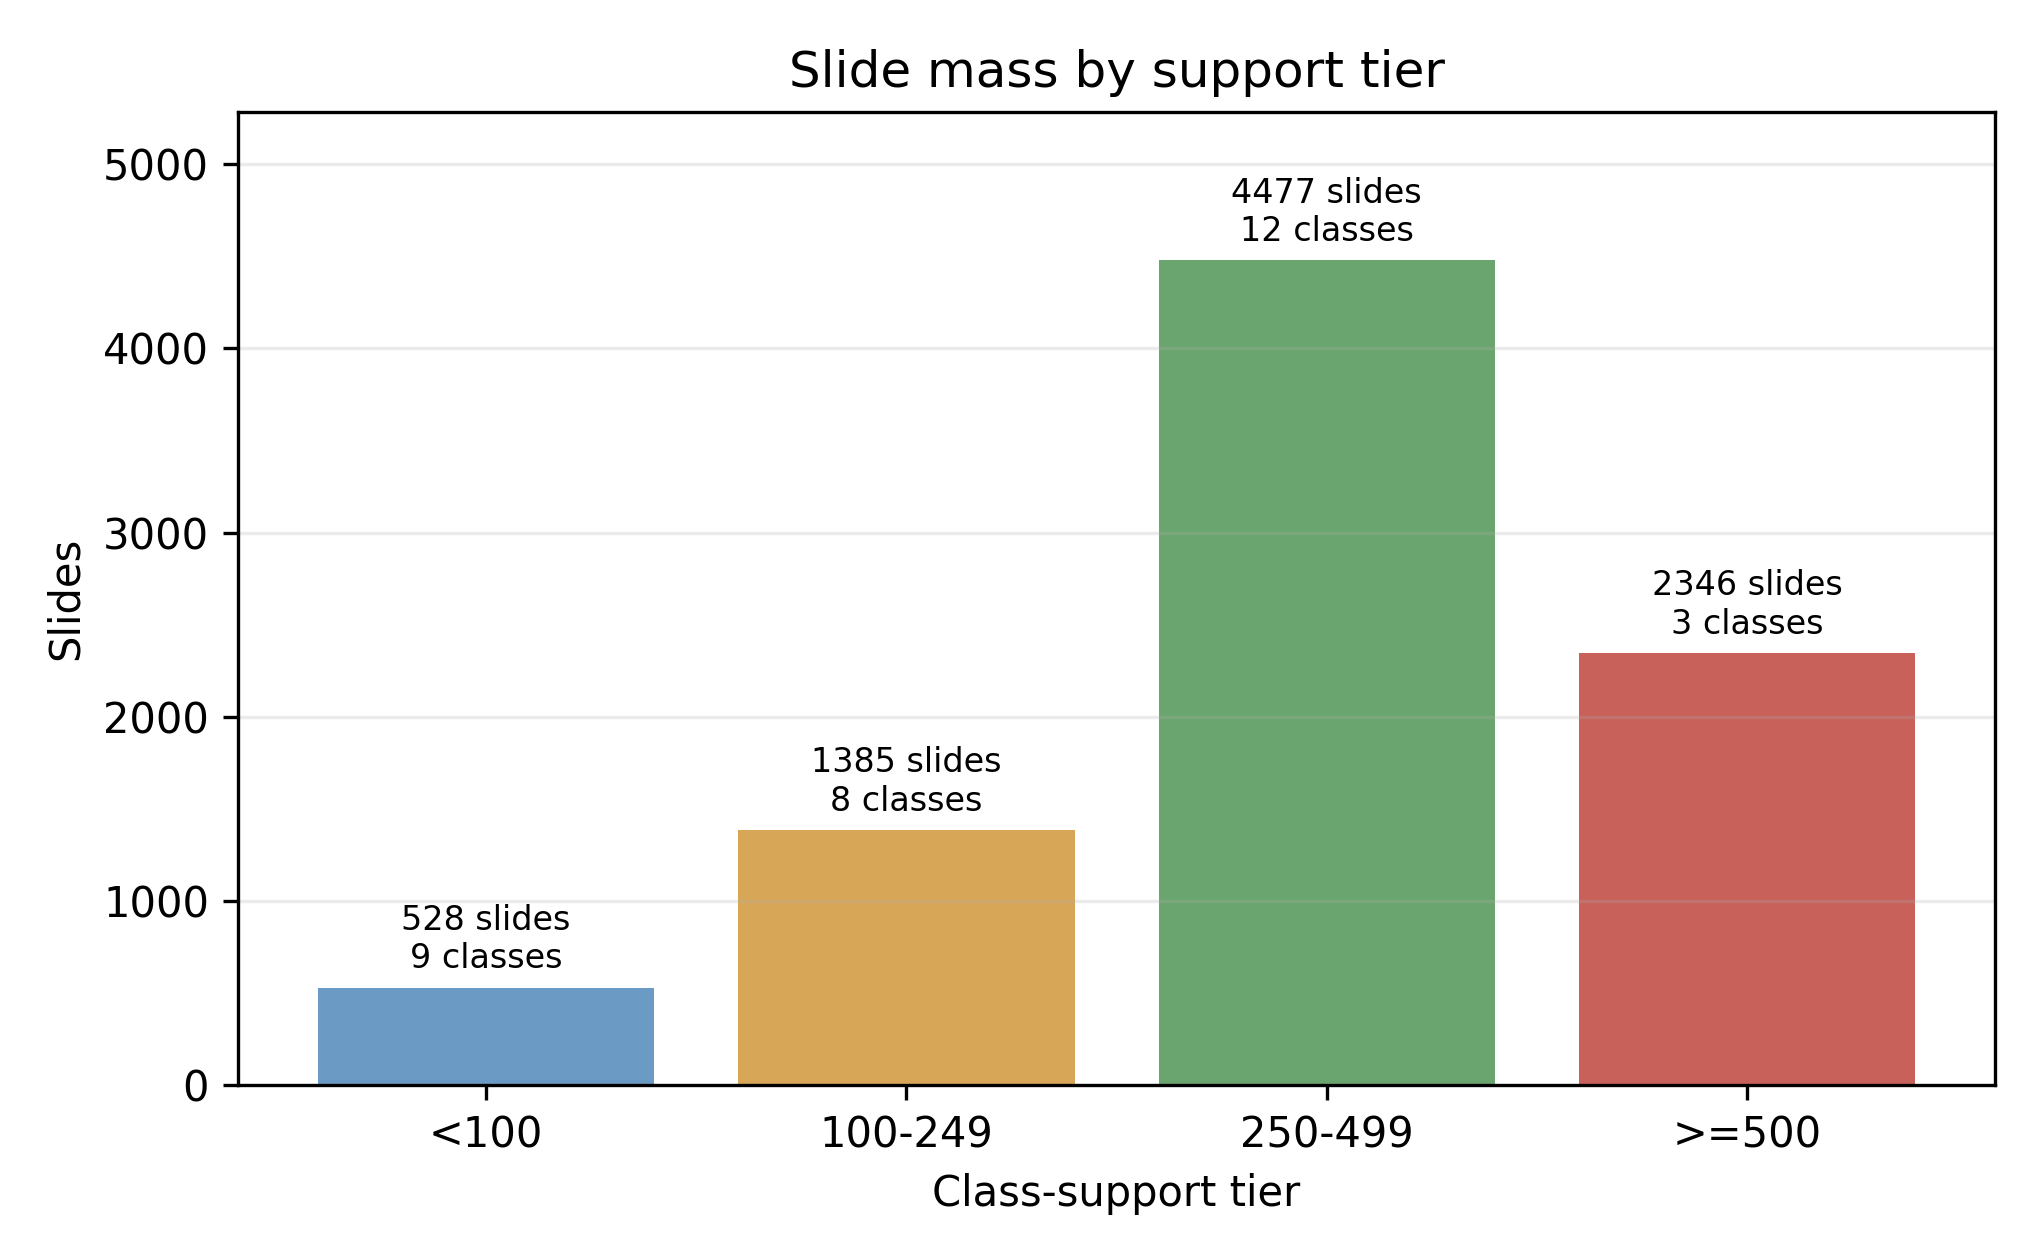
\includegraphics[width=0.7\linewidth]{long_tail_profile.png}}{\fbox{\parbox{0.7\linewidth}{Long-tail profile generated by \texttt{scripts/prep/explore.py}.}}}
  \caption{Class-rank profile used to verify the long-tailed setting.}
  \label{fig:long-tail}
\end{figure}

\section{Mitigation Taxonomy}
The experiments follow five method families. Data-level methods change which examples are shown during training, including oversampling and class-balanced sampling \citep{majeed2024addressingData}. Synthetic and generative methods create new minority-class examples; full image-level GAN or diffusion training is discussed as related work, while this experiment remains feature-based for comparability \citep{yuan2024aGan,ruizcasado2024enhancingHistopathological}. Algorithm-level methods change the objective through class weights, focal loss, or center/prototype regularization \citep{mahbub2024centerFocused}. Hybrid methods combine sampling and objective changes \citep{ling2025mdeMil}. Representation and architecture-level methods improve separability through model design or set-level supervision \citep{cong2022imbalancedHistopathology,muttenthaler2024oko}.

\section{Methods}
All methods consume the same native TCGA-UT Virchow2 feature manifest. The baseline is a multilayer perceptron trained with unweighted cross-entropy. Feature-space probes use $k$-nearest neighbors and nearest-centroid classification. Sampling variants use class-balanced replacement sampling. Objective variants use inverse-frequency weighting, focal loss, weighted focal loss, and a center-regularized cross-entropy variant. Hybrid variants combine balanced sampling with weighted focal loss. A set-learning variant trains on odd-$k$-out sets and evaluates the same single-example classifier at test time.

The main evaluation uses native validation and test distributions. The primary metrics are macro F1, balanced accuracy, and classwise recall ordered by class support. These metrics are chosen because accuracy and ROC-style summaries can overstate performance under class imbalance \citep{mosquera2024classImbalance}.

\section{Results}
Table~\ref{tab:summary} summarizes aggregate test performance once the training jobs complete. Figure~\ref{fig:method-summary} compares macro F1 across methods, and Figure~\ref{fig:classwise-recall} shows whether improvements are concentrated in rare classes or distributed across the class spectrum.

\begin{table}[ht]
  \centering
  \caption{Aggregate method results. Generated from \texttt{outputs/tables/result\_summary.csv}.}
  \label{tab:summary}
  \IfFileExists{../outputs/tables/result_summary.tex}{\begin{tabular}{lccc}
\toprule
Method & Balanced accuracy & Macro F1 & Split\\
\midrule
center\_ce & 0.856 & 0.869 & test\\
weighted\_ce & 0.845 & 0.846 & test\\
feature\_interpolation\_ce & 0.844 & 0.845 & test\\
ce & 0.847 & 0.845 & test\\
focal & 0.842 & 0.844 & test\\
weighted\_focal & 0.848 & 0.840 & test\\
oversampling\_ce & 0.842 & 0.840 & test\\
balanced\_sampler\_weighted\_focal & 0.852 & 0.840 & test\\
balanced\_sampler\_ce & 0.847 & 0.837 & test\\
knn & 0.768 & 0.769 & test\\
oko & 0.771 & 0.712 & test\\
ncc & 0.734 & 0.686 & test\\
\bottomrule
\end{tabular}
}{\begin{tabular}{lccc}\toprule Method & Balanced accuracy & Macro F1 & Notes\\ \midrule Pending & -- & -- & Run aggregation first.\\ \bottomrule\end{tabular}}
\end{table}

\begin{figure}[ht]
  \centering
  \IfFileExists{../outputs/figures/method_macro_f1_test.png}{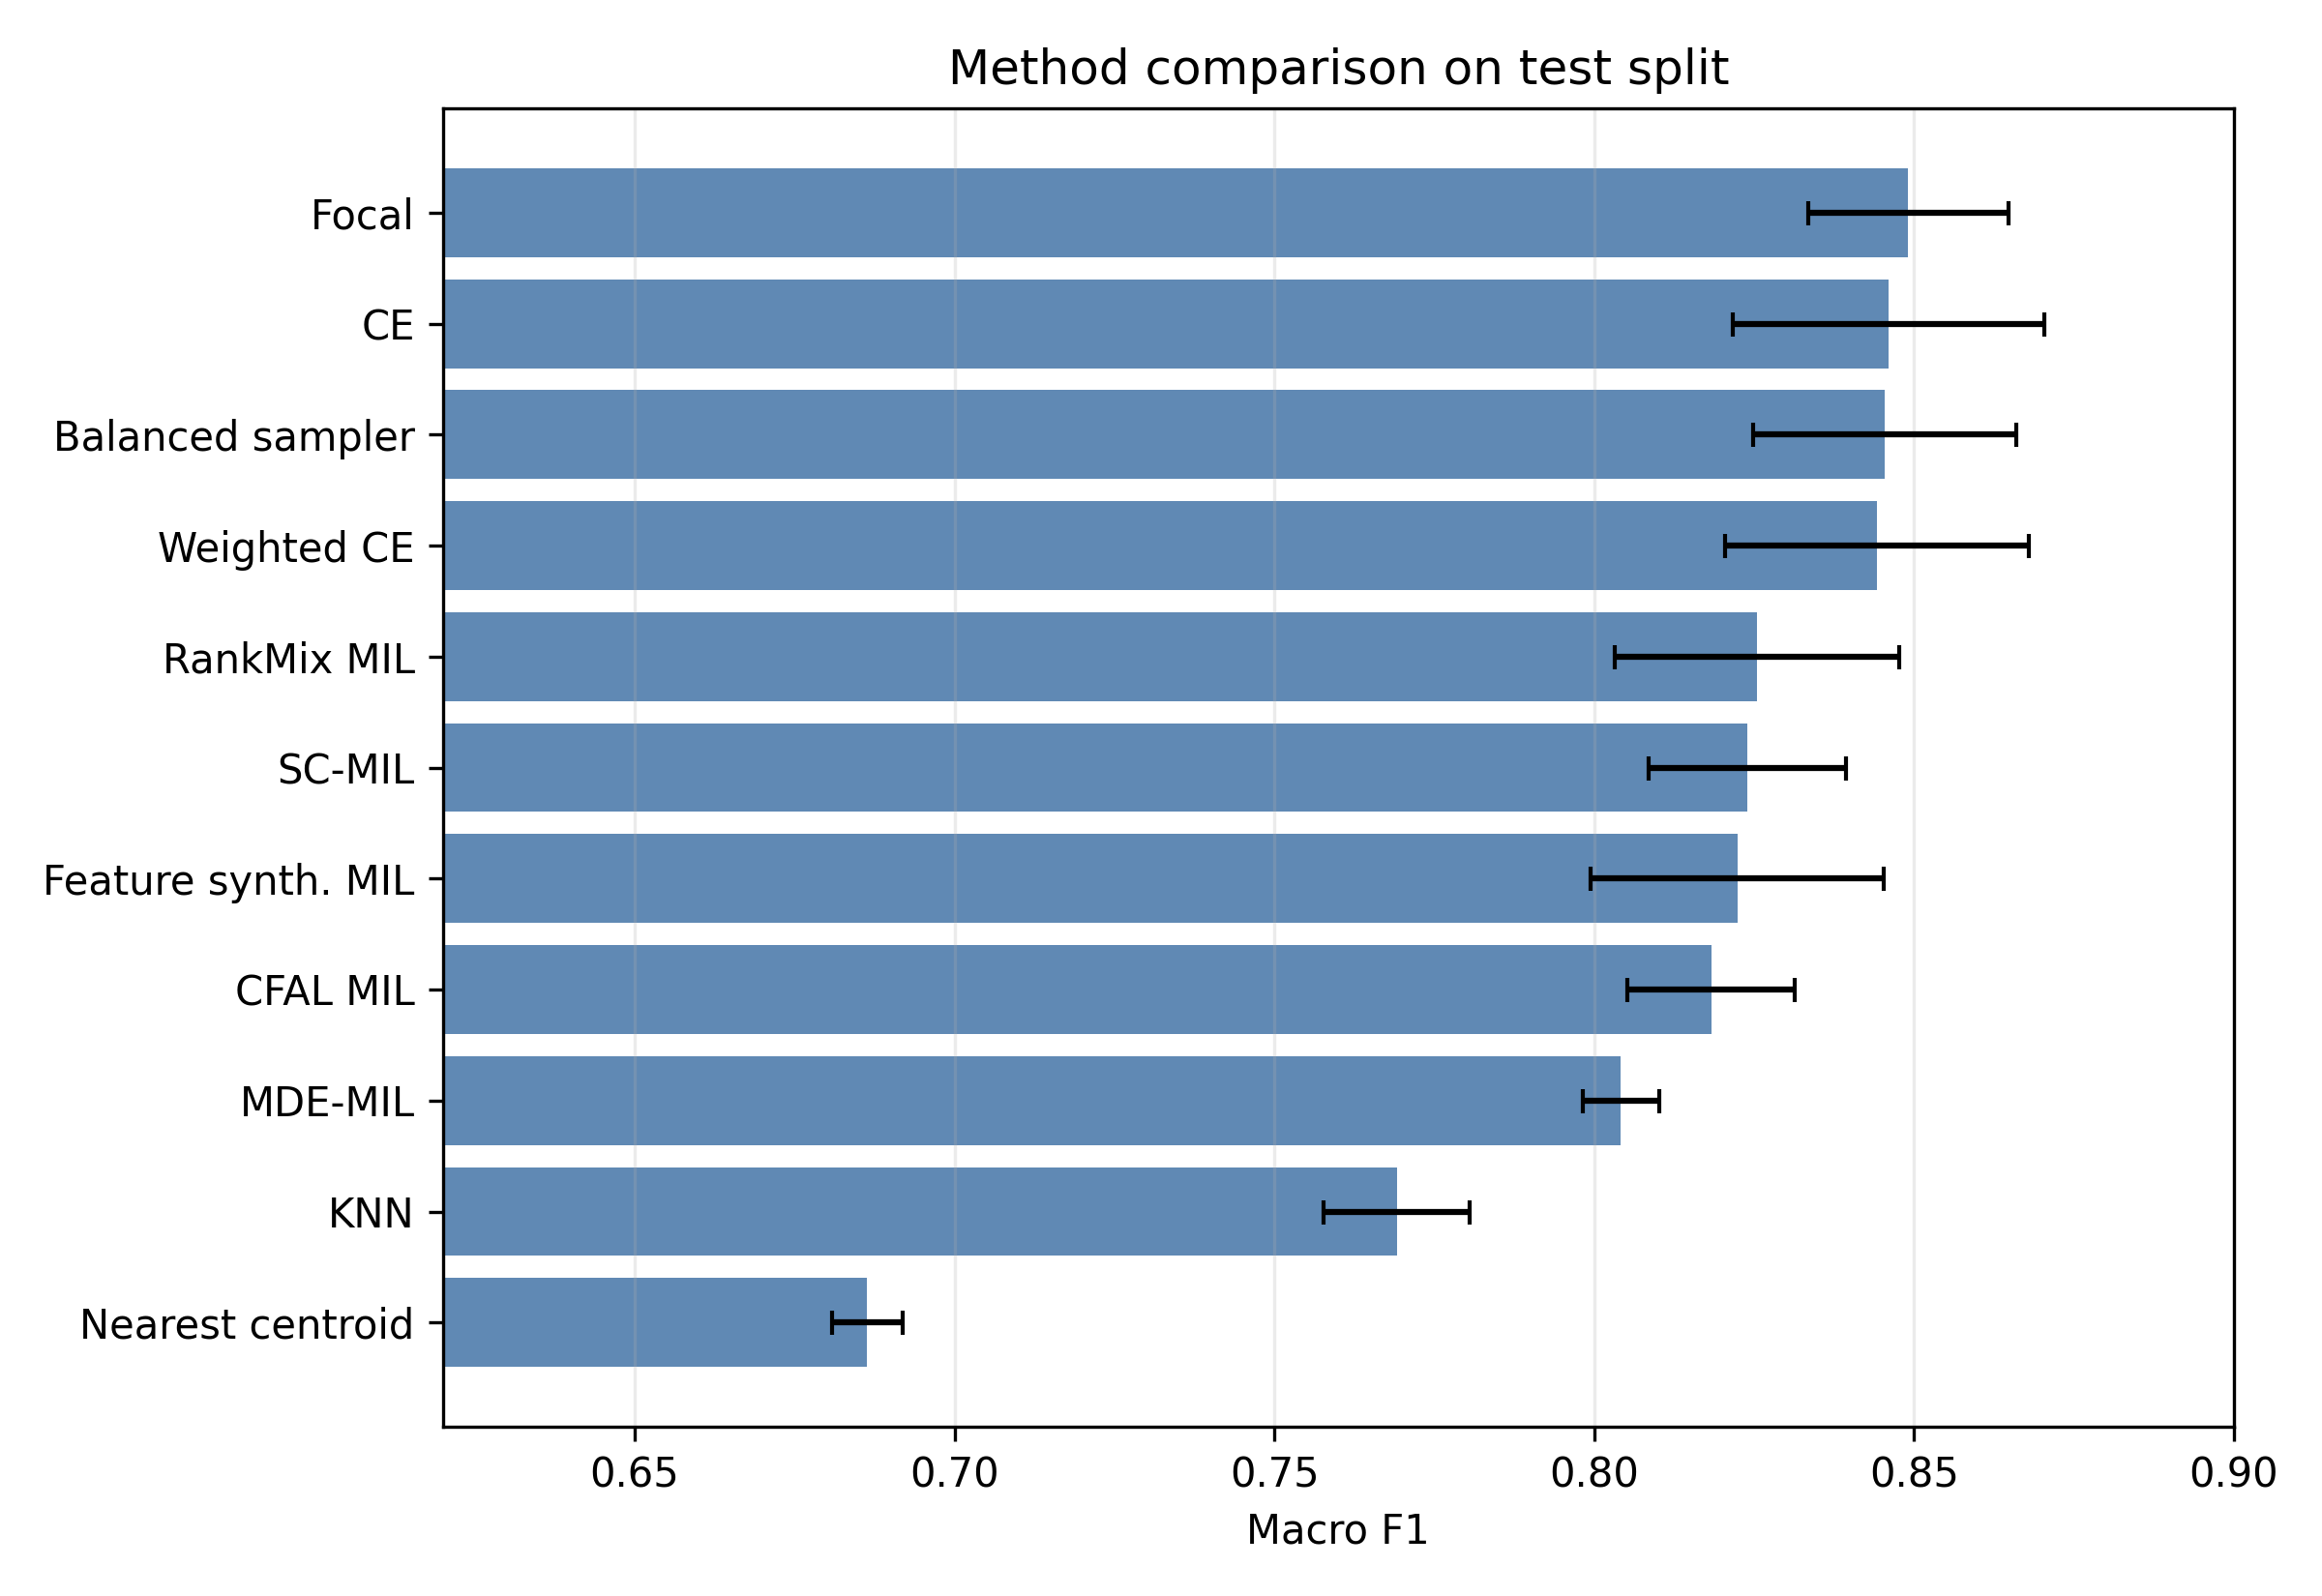
\includegraphics[width=0.8\linewidth]{method_macro_f1_test.png}}{\fbox{\parbox{0.8\linewidth}{Method summary generated by \texttt{scripts/report/figures.py}.}}}
  \caption{Macro F1 by mitigation method on the native test distribution.}
  \label{fig:method-summary}
\end{figure}

\begin{figure}[ht]
  \centering
  \IfFileExists{../outputs/figures/classwise_recall_test.png}{
\includegraphics[width=\linewidth]{classwise_recall_test.png}}{\fbox{\parbox{0.85\linewidth}{Classwise recall generated by \texttt{scripts/report/figures.py}.}}}
  \caption{Classwise recall by method, ordered by test support.}
  \label{fig:classwise-recall}
\end{figure}

\section{Discussion}
The expected comparison is not only which method maximizes macro F1, but how each method trades minority-class recall against majority-class stability. Sampling methods should improve minority exposure but can increase variance. Loss weighting and focal losses change the optimization signal without deleting majority examples. Hybrid methods may help when both exposure and objective imbalance matter, but they can overcorrect. Feature-space synthetic augmentation is interpreted cautiously because it is not equivalent to validated image-level generative pathology synthesis.

\section{Conclusion}
This experiment package provides a reproducible workflow for studying class-imbalance mitigation on native TCGA-UT using a shared frozen feature representation. The resulting paper should report both aggregate metrics and classwise behavior so that gains for rare classes are not hidden by the head of the distribution.

\bibliographystyle{plainnat}
\bibliography{references}

\end{document}

